%%
%% --------------------------------------------------------------
%% --------------------------------------------------------------

\section{Presentación de la asignatura}

%%---------------------------------------------------------------

\begin{frame}
\frametitle{Datos, datos, datos}

\begin{itemize}
\item Profesores:
  \begin{itemize}
  \item Jesús M. González Barahona (jgb @ gsyc.urjc.es)
  \item Gregorio Robles (grex @ gsyc.urjc.es)
  \item David Moreno Lumbreras (david.morenolu @ urjc.es)
  \item Alberto Rodríguez Iglesias (alberto.rodriguezi @ urjc.es)
  \item Alberto García ( @ urjc.es)
  \item Sergio Montes (sergio.montes @ urjc.es)
  \end{itemize}
\item Grupo de Sistemas y Comunicaciones (GSyC)
\item Horario: \horario
\item Tutoría: Horario por definir (via videoconferencia)
%\item Laboratorio 209 Laboratorios III
\end{itemize}

\begin{flushright}
  Clases: Laboratorios III, \labo \\
  Campus virtual: {\small \url{http://aulavirtual.urjc.es}} \\
  Cursos web: {\small \url{http://cursosweb.github.io}} \\
  GitLab de la EIF: {\small \url{http://gitlab.eif.urjc.es}} \\
\end{flushright}

\end{frame}


%-----------------------    ---------------------------------
\usebackgroundtemplate{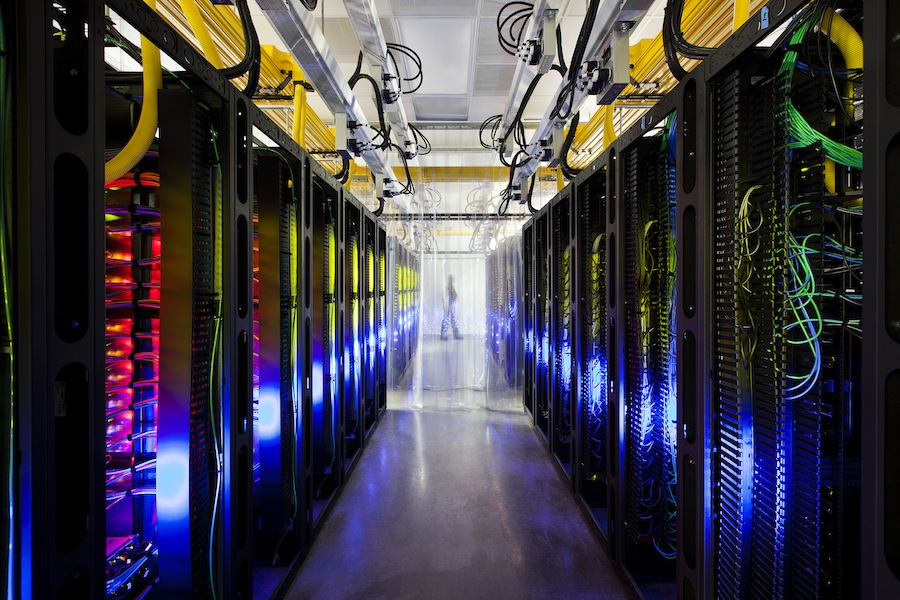
\includegraphics[width=12.8cm]{figs/internet.jpg}}
% http://cdn6.yorokobu.es/wp-content/uploads/Council-Bluffs-Network-Room.jpg

\begin{frame}
\frametitle{¿De qué va todo esto?}

\vspace{3.5cm}

\begin{center}
\color{white}
\Huge {\bf Entendiendo cómo funciona la web}
\end{center}

\end{frame}
\usebackgroundtemplate{}


%%---------------------------------------------------------------

\begin{frame}
\frametitle{En concreto...}

{\Large
\begin{itemize}
\item Cómo se construyen los sistemas reales \\
  que se usan en Internet
  \item Qué tecnologías se están usando
  \item Qué esquemas de seguridad hay
  \item Cómo encajan las piezas
  \item En la medida de lo posible, ``manos en la masa''
\end{itemize}
}

\end{frame}


%%---------------------------------------------------------------

\begin{frame}
\frametitle{Ejemplos}

{\Large
\begin{itemize}
  \item ¿Qué es una aplicación web?
  \item ¿Qué es una sesión?
  \item ¿Cómo construir un servicio REST?
  \item Acaba con la magia de los servicios web
  \item ¿Cómo se hace un servicio basado en contenidos?
\end{itemize}
}
\end{frame}

%-----------------------    ---------------------------------
\usebackgroundtemplate{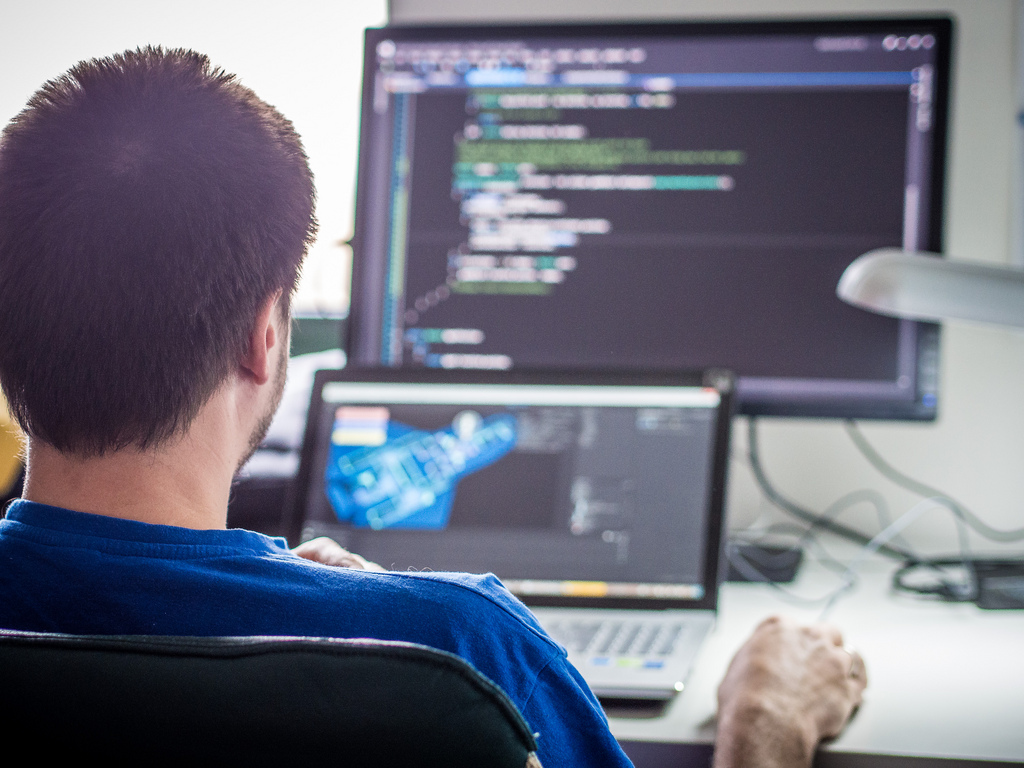
\includegraphics[width=13cm]{figs/programmer.jpg}}
% http://www.openweigh.com/assets/programmer-e898f9c9a43ecd208f1f1df347713e6e.jpg

\begin{frame}
\frametitle{Fundamentos de la asignatura}

\vspace{3.8cm}

\begin{center}
\color{red}
\Huge {\bf La programación es el lenguaje de la tecnología}
\end{center}

\end{frame}
\usebackgroundtemplate{}

%-----------------------    ---------------------------------

\begin{frame}
\frametitle{Lenguaje de Programación: Python}

\begin{center}
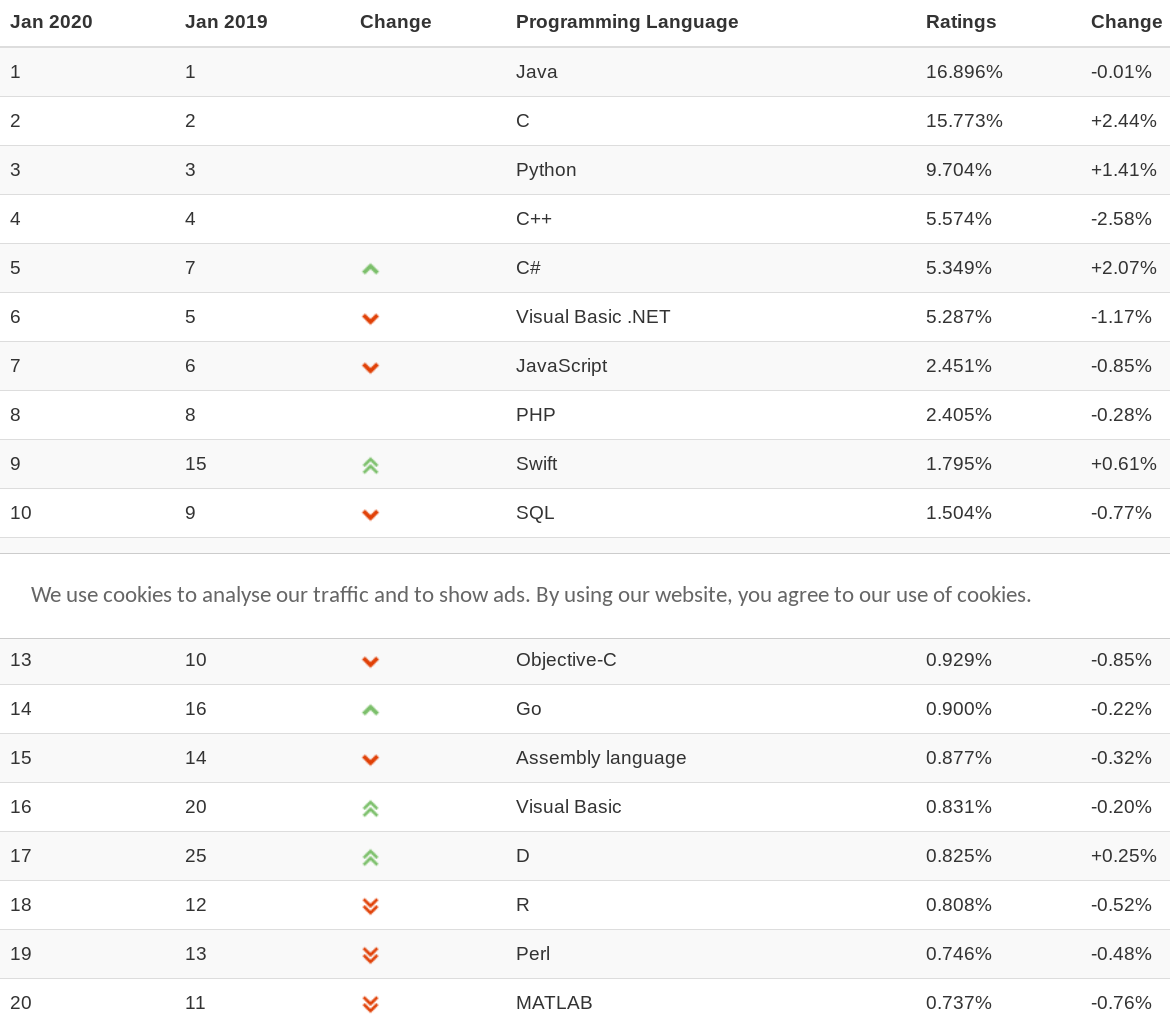
\includegraphics[width=5cm]{figs/2020-most-popular-lang-tiobe}
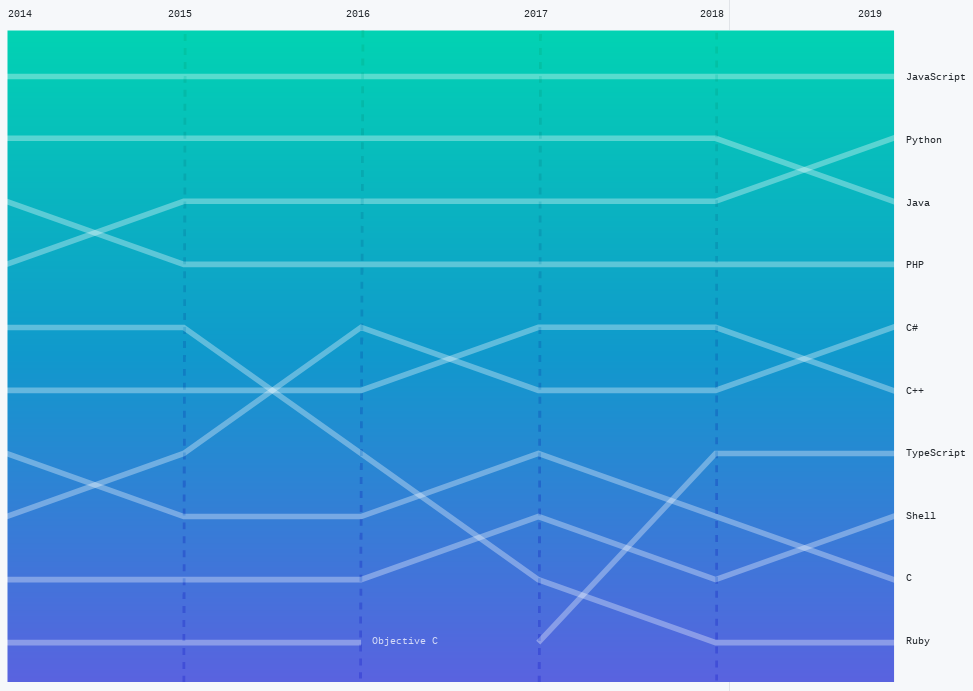
\includegraphics[width=6cm]{figs/2019-most-popular-lang-github}
\end{center}

\begin{center}
  {\Large Primer Mandamiento: \\ Amarás Python por encima de (casi) todo.} \\
  TIOBE (enero 2020) ~~~~ GitHub (noviembre 2019) \\
\end{center}

\begin{flushright}
  \url{https://www.youtube.com/watch?v=UNSoPa-XQN0}
\end{flushright}
\end{frame}
\usebackgroundtemplate{}


%-----------------------    ---------------------------------

\begin{frame}
\frametitle{Plataforma: Django}

\begin{center}
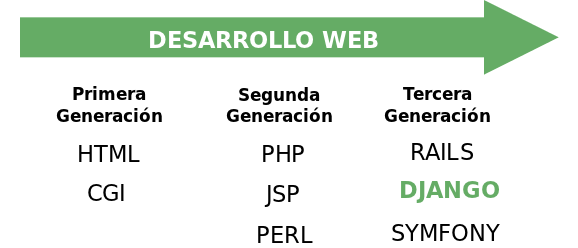
\includegraphics[width=11cm]{figs/django.png}
% http://www.maestrosdelweb.com/images/2012/04/desarrolloweb.png
\end{center}

\begin{center}
\Large Segundo Mandamiento: \\ No tomarás el nombre de Django en vano.
\end{center}


\end{frame}
\usebackgroundtemplate{}

%-----------------------    ---------------------------------

\begin{frame}
\frametitle{Plataforma: Django (2)}

{\large Algunas referencias a principales marcos de desarrollo web (2025):}

\vspace{0.5cm}

\begin{itemize}
\item ``10 Software Development Frameworks That Will Dominate 2025'' \\
  {\small \url{https://www.index.dev/blog/10-programming-frameworks}}
\item ``Web Application Development | Top 10 Frameworks in 2025'' \\
  {\small \url{https://www.sencha.com/blog/web-application-development-top-frameworks/}}
\item ``The Top 10 Frameworks for Web Development in 2025'' \\
  {\small \url{https://medium.com/@technosoftwares21/the-top-10-frameworks-for-web-development-in-2025-4a7fc54f47dc}}
\end{itemize}

\vspace{1cm}
{\large Suele ser el preferido en Python, y uno de los 10 principales.}

\end{frame}

%%---------------------------------------------------------------

\begin{frame}
\frametitle{Metodología}

{\Large
  \begin{center}
    Objetivo principal: \\
    conceptos básicos de construcción de sitios web modernos \\
  \end{center}

  \vspace{0.5cm}
\begin{itemize}
\item Clases de teoría y de prácticas, pero...
\item Teoría en prácticas, prácticas en teoría
\item Uso de resolución de problemas para aprender
\item Construcción de un proyecto a lo largo del curso
\end{itemize}

  \vspace{0.5cm}

\begin{center}
  Fundamentalmente, entender lo fundamental
\end{center}
}
\end{frame}

%-----------------------    ---------------------------------
\usebackgroundtemplate{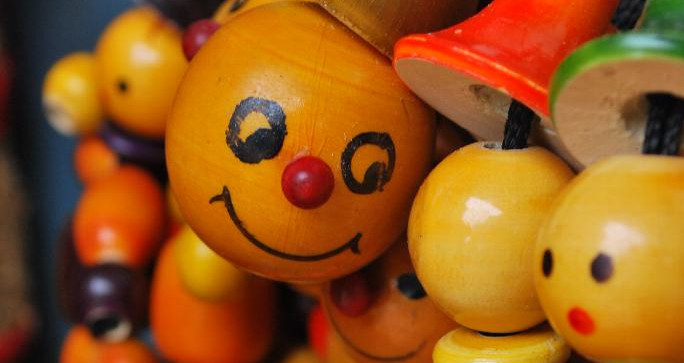
\includegraphics[width=13cm]{figs/toys.jpg}}

\begin{frame}
\frametitle{Fundamentos de la asignatura}

\vspace{5.4cm}

\begin{center}
  \Huge Aprender no puede ser aburrido
\end{center}

\end{frame}
\usebackgroundtemplate{}

%-----------------------    ---------------------------------
\usebackgroundtemplate{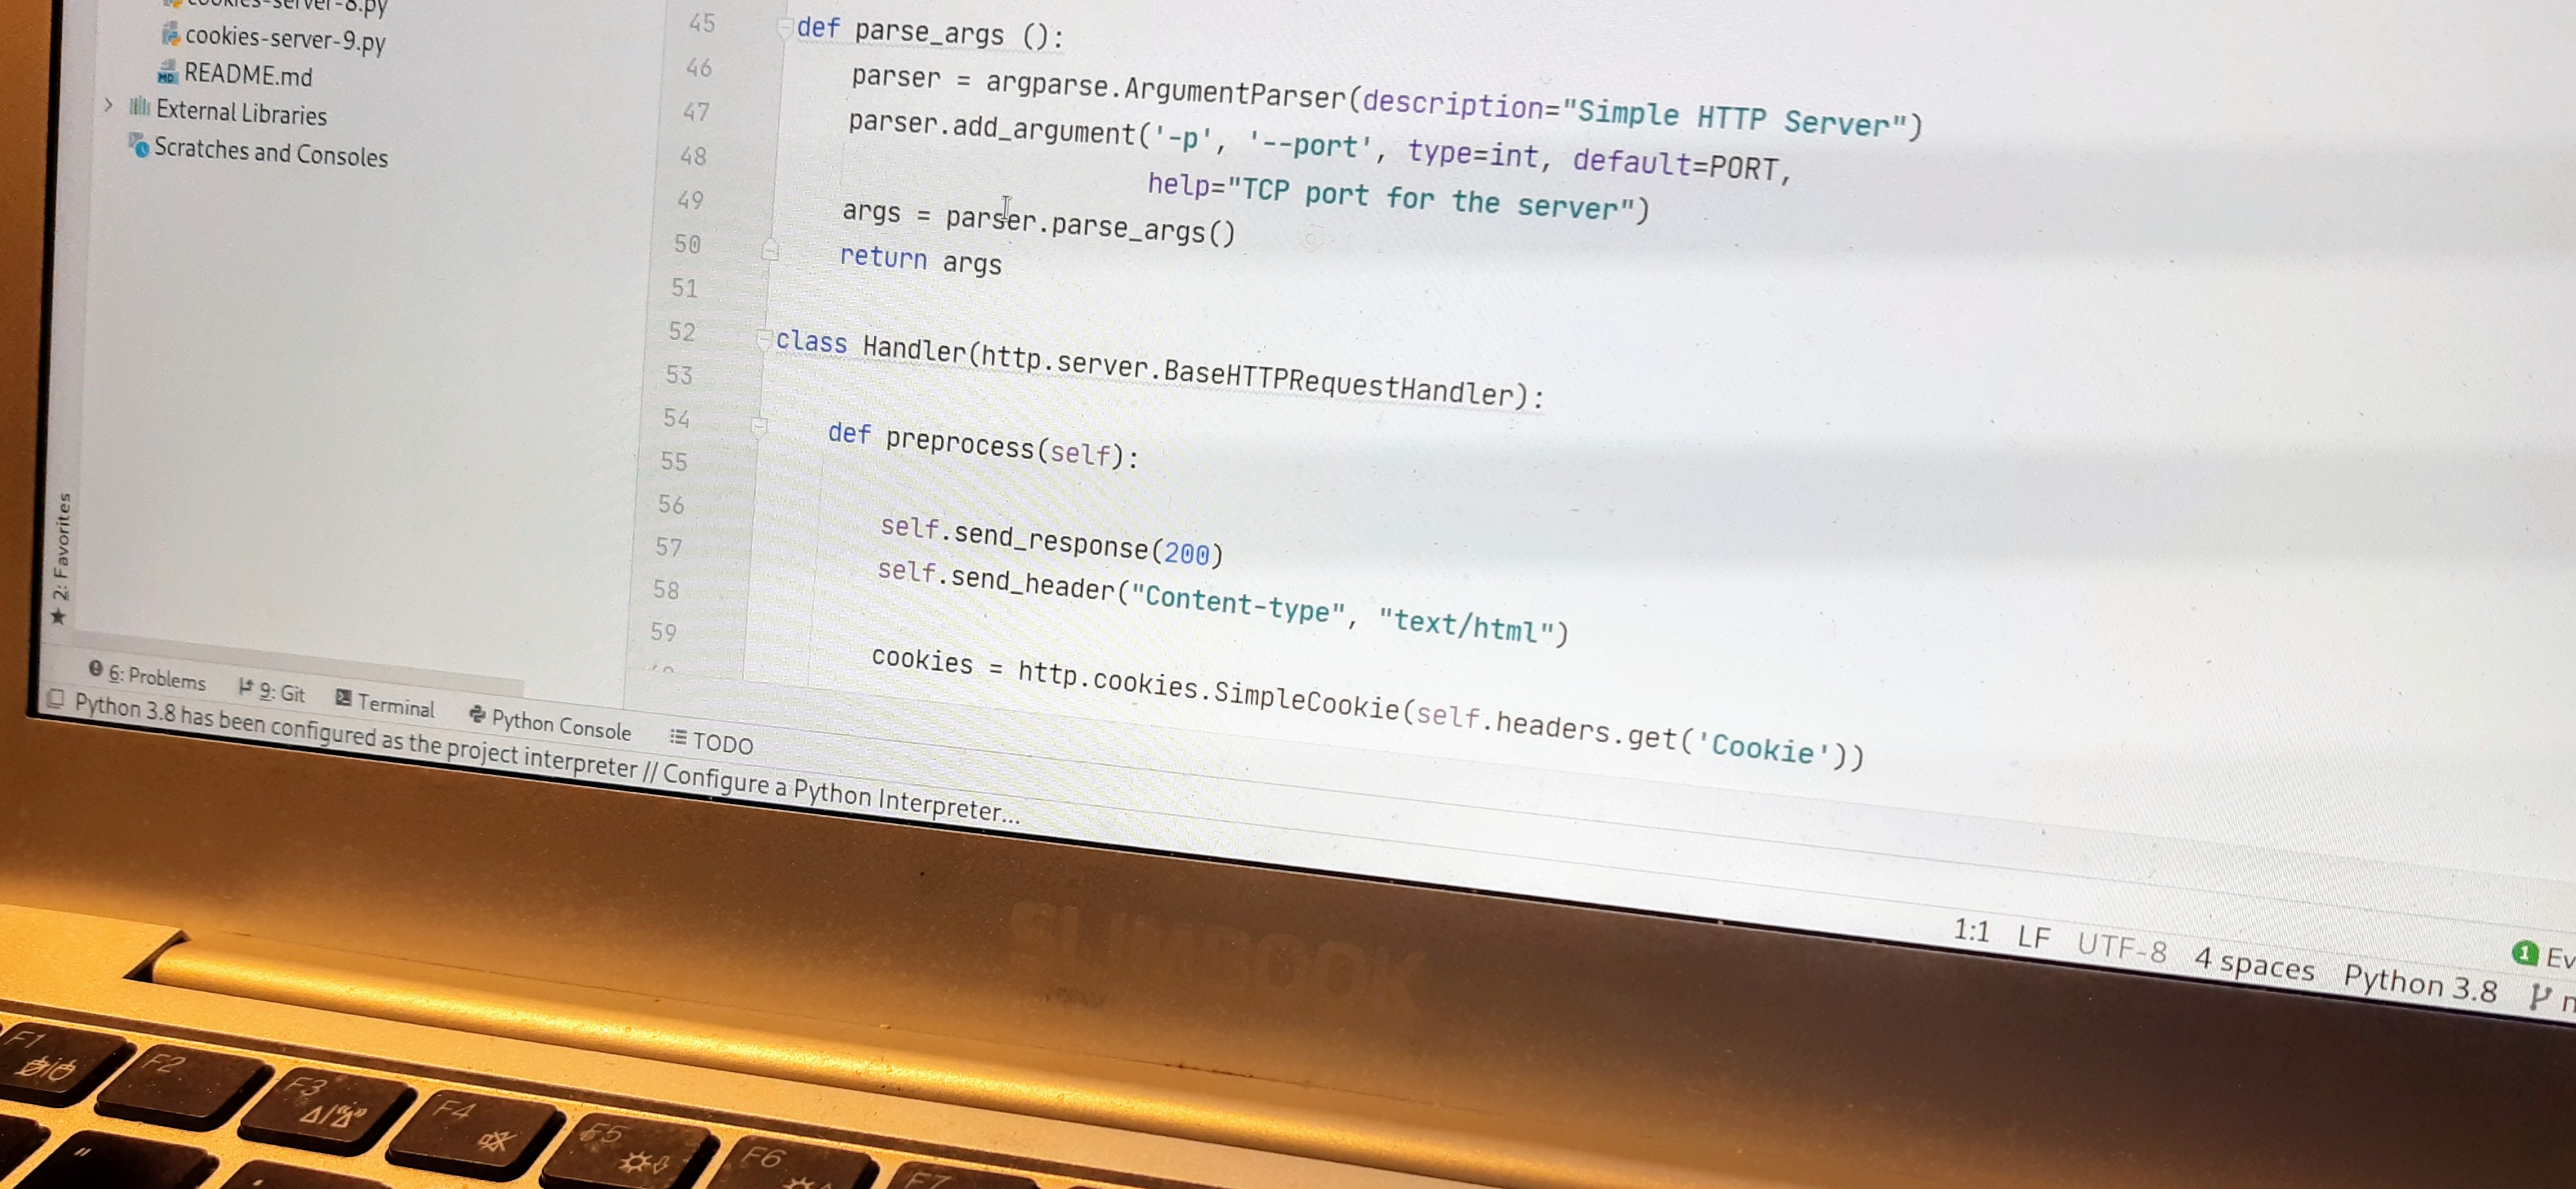
\includegraphics[width=13cm]{figs/code.jpg}}

\begin{frame}
\frametitle{Fundamentos de la asignatura(2)}

\vspace{5.4cm}

\begin{center}
  \Huge La letra con código entra
\end{center}

\end{frame}
\usebackgroundtemplate{}
%%---------------------------------------------------------------

\begin{frame}
\frametitle{Las Clases}

\begin{itemize}
  \item Empezamos en punto
  \item A veces: 5--10 min. de Frikiminutos
  \begin{itemize}
    \item Gadgets tecnológicos
    \item Aplicaciones
    \item Cuestiones interesantes
    \item \dots
  \end{itemize}
  \item A veces, explicación de los conceptos más importantes y luego
    realización de ejercicios
  \item A veces, al revés
  \item Ejercicios para hacer fuera de clase (y entregar)
\end{itemize}

\end{frame}



%-----------------------    ---------------------------------
\usebackgroundtemplate{
\includegraphics[width=13.5cm]{figs/challenge.jpg}}
% http://ichallenge.com/wp-content/uploads/2014/08/challenge-6.jpg

\begin{frame}
\frametitle{Fundamentos de la asignatura}

\vspace{-2.75cm}

\begin{center}
\Huge El estudiante es el centro del aprendizaje
\end{center}

\end{frame}
\usebackgroundtemplate{}

%-----------------------    ---------------------------------
\usebackgroundtemplate{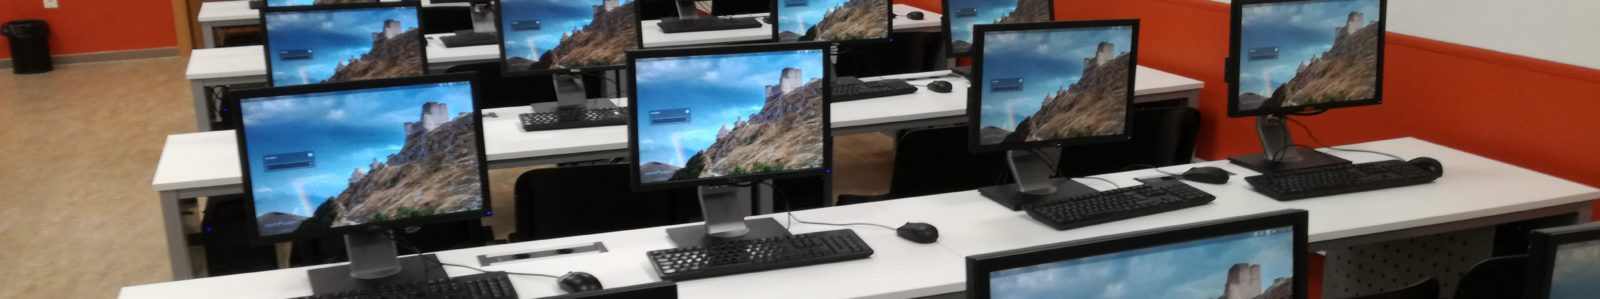
\includegraphics[width=13.5cm]{figs/labo.jpg}}
\begin{frame}
\frametitle{Laboratorio}

~
\vspace{1cm}

\begin{itemize}
\item Laboratorios Linux de la EIF
\item Este curso, a distancia: vía VNC, vía ssh...
\item \url{https://labs.eif.urjc.es}
\end{itemize}

\vspace{1cm}

Software (fundamental) que utilizaremos:

\begin{itemize}
\item Ubuntu
\item Python, Django
\item PyCharm
\end{itemize}
\end{frame}
\usebackgroundtemplate{}


%%---------------------------------------------------------------

\begin{frame}
\frametitle{Evaluación}

\begin{itemize}
\item Microprácticas diarias (entrega foro/GitLab): 0 a 1
\item Miniprácticas preparatorias: 0 a 1
\item Proyecto final (obligatorio): 0 a 2.
\item Opciones y mejoras práctica final: 0 a 3
\item Teoría (obligatorio): 0 a 4. \\
  \hspace{.5cm} Ojo: teoría fuertemente relacionada con prácticas
\item Nota final: Suma de notas, moderada por la interpretación del profesor
\item Mínimo para aprobar:
      \begin{itemize}
      \item Aprobado en teoría (2) y proyecto final (1), y
      \item 5 puntos de nota final en total
      \end{itemize}
\end{itemize}

\end{frame}

%%---------------------------------------------------------------

\begin{frame}
\frametitle{Evaluación (2)}

\begin{itemize}
\item Evaluación teoría: prueba escrita (quizás en ordenador)
\item Microprácticas diarias y miniprácticas incrementales:
      \begin{itemize}
      \item es muy recomendable hacerlas
      \end{itemize}
\item Evaluación proyecto final
      \begin{itemize}
      \item posibilidad de examen presencial para proyecto final
      \item ¡tiene que funcionar en el laboratorio!
      \item enunciado mínimo obligatorio supone 1, se llega a 2 sólo con calidad y cuidado en los detalles
      \end{itemize}
\item Opciones y mejoras proyecto final:
      \begin{itemize}
      \item permiten subir mucho la nota
      \end{itemize}
\item Evaluación extraordinaria:
  \begin{itemize}
  \item prueba escrita (si no se aprobó la ordinaria)
  \item nuevo proyecto final (si no se aprobó el ordinario)
  \end{itemize}
\end{itemize}
\end{frame}


%%---------------------------------------------------------------

\begin{frame}
 \frametitle{Proyecto final}

Ejemplos del pasado:

\begin{itemize}
 \item Servicio de búsqueda de hoteles
 \item Servicio de apoyo a la docencia
 \item Sitio de intercambio de fotos
 \item Aplicación web de autoevaluación docente
 \item Agregador de blogs (canales RSS)
 \item Agregador de microblogs (Identi.ca, Twitter)
\end{itemize}

\end{frame}

%%---------------------------------------------------------------

\begin{frame}
 \frametitle{Proyecto final}

Este curso...

\vspace{1cm}

\begin{center}
  \Huge ....
\end{center}
\end{frame}


%%---------------------------------------------------------------

\begin{frame}
\frametitle{Ejemplos de prácticas finales de otros años}

\begin{itemize}
\item Niki Montero (2024): \\ \url{https://www.youtube.com/watch?v=coAf8o0gQ00}
\item Ainhoa Hernández (2021: \\ \url{https://www.youtube.com/watch?v=7Bd33IS3XBE}
\item Noelia López (2019): \\ \url{https://youtube.com/watch?v=VRg37vwUll0}
%\item Felipe Cordente (2019): \\ \url{https://www.youtube.com/watch?v=TfI9MaA4IV0}
%\item Daniel Arévalo (2019): \\ \url{https://www.youtube.com/watch?v=TfI9MaA4IV0}
\item Fernando Yustas (2014):\\ \url{https://youtube.com/watch?v=TUUMVEaBzeg}
%\item Miguel Ariza (2014): \\ \url{https://youtube.com/watch?v=fVBx9cGPjWs}
\end{itemize}

(puedes buscar en YouTube muchos más ejemplos)

\end{frame}



%%---------------------------------------------------------------

\begin{frame}
\frametitle{¡Ánimo!}

\begin{center}
{\huge Aquí se enseñan cómo son las cosas \\
  que se usan en el mundo real \\
  ~ \\
  Las buenas noticias son\dots \\
  que no son tan difíciles\\}
\end{center}

\end{frame}



